\renewcommand{\theequation}{\theenumi}
\renewcommand{\thefigure}{\theenumi}
\begin{enumerate}[label=\thesection.\arabic*.,ref=\thesection.\theenumi]
\numberwithin{equation}{enumi}
\numberwithin{figure}{enumi}
%
\item Suppose you drop a die at random on the rectangular region shown in Fig. \ref{fig:chapters/uniform/1/}. What is the probability that it will land inside the circle with diameter 1m?
\begin{figure}[!ht]
\centering
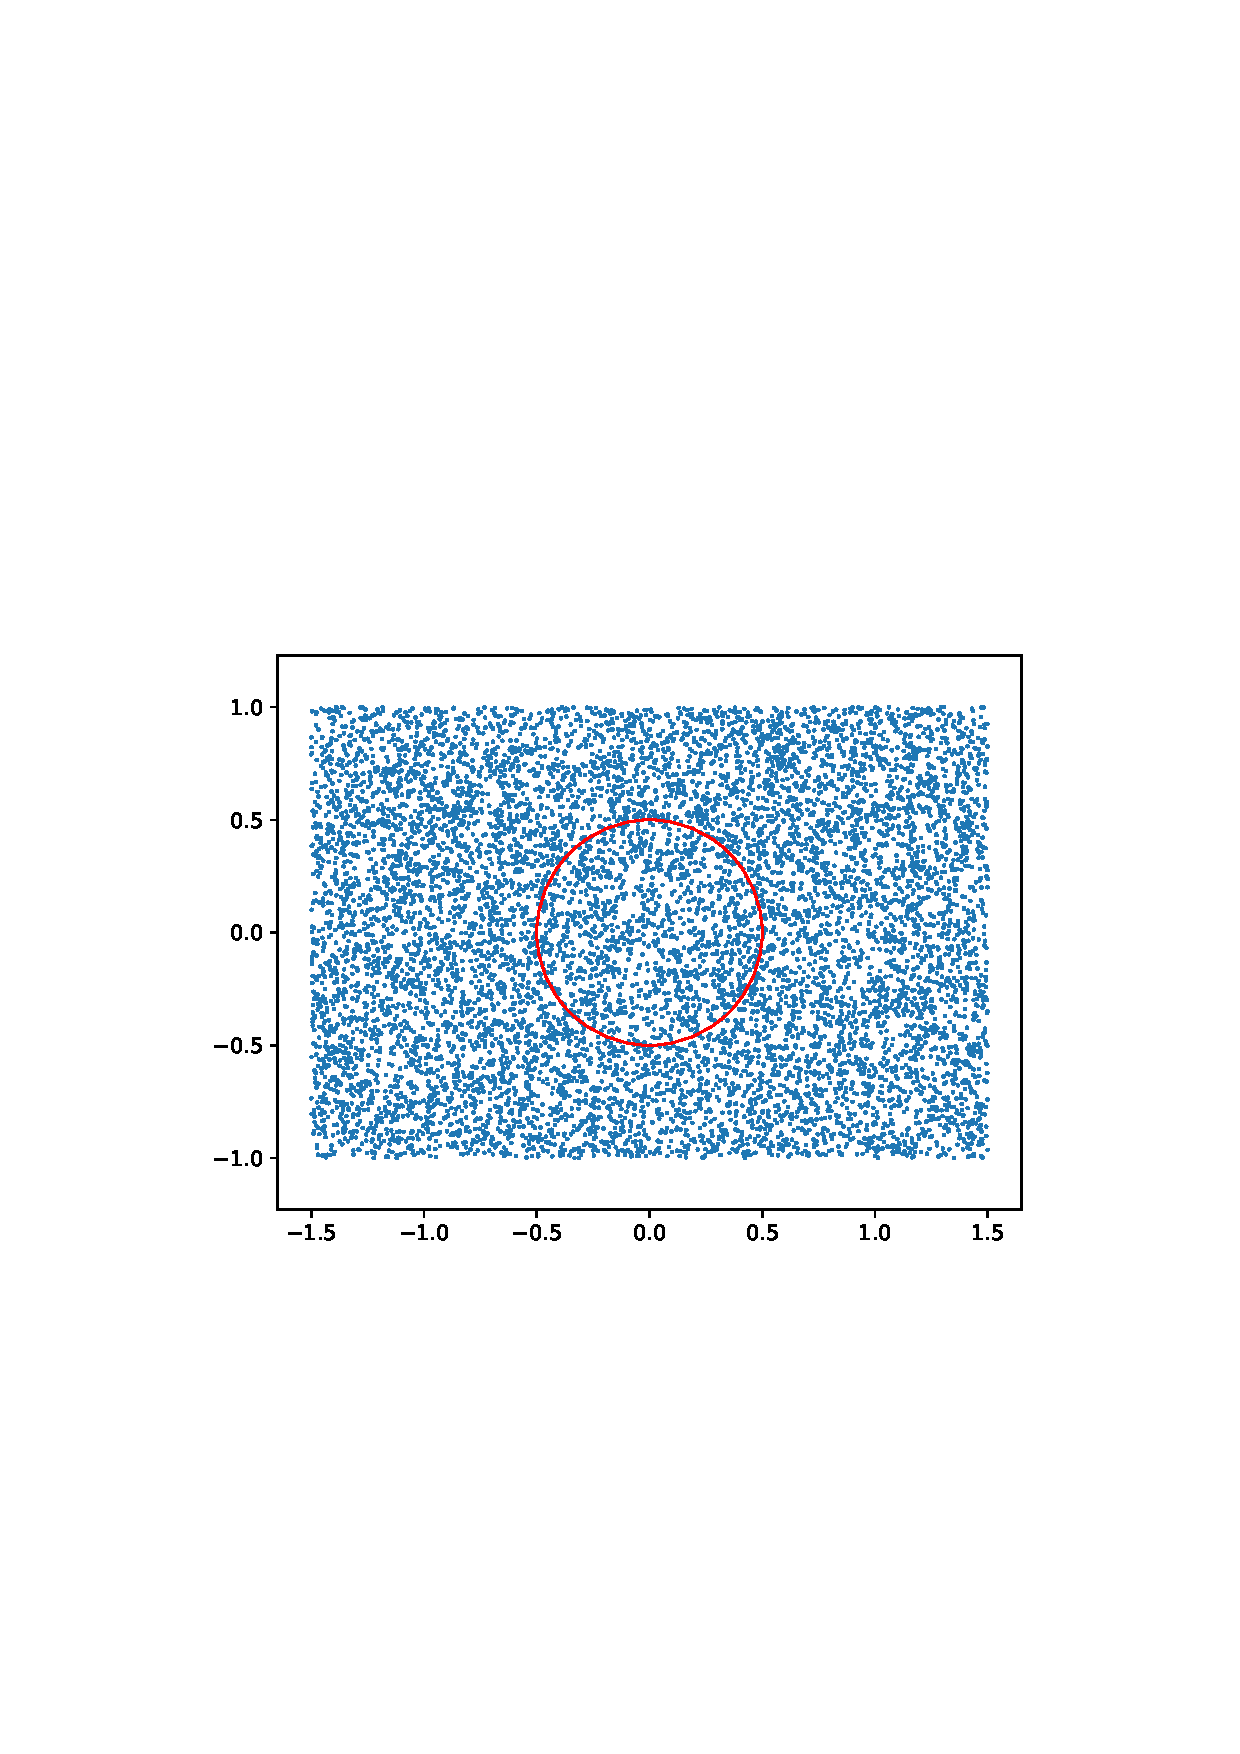
\includegraphics[width=\columnwidth]{./figs/uniform/rectangle.png}
\caption{}
\label{fig:chapters/uniform/1/}
\end{figure}
\\
\solution
In Fig. \ref{fig:chapters/uniform/1/}, the sample size $S$ is the area of the rectangle given by 
\begin{align}
S=3x2=6 m^2
\end{align}
The event size is the area of the circle given by 
\begin{align}
E = \pi\brak{\frac{1}{2}}^2=\frac{\pi}{4} m^2 
\end{align}
The probabilty of the dice landing in the circle is
\begin{align}
\pr{E} = \frac{E}{S} = \frac{\pi}{24}
\label{eq:chapters/uniform/1/prob}
\end{align}
%
The python code is available in 
\begin{lstlisting}
/codes/uniform/rect.py
\end{lstlisting}
The python code generates 10,000 points uniformly within the rectangle of dimensions $3 \times 2$ and checks for the number of points within the circle of radius 0.5.  The ratio of these is close to $\frac{\pi}{24}$.  Note that each time the code is run, the ratio will change, but will still be close to $\frac{\pi}{24}$.

%In general, the complex number $\myvec{a_1\\a_2}$ has the matrix representation
\begin{align}
\label{eq:3.4.1_Complex}
\myvec{a_1\\a_2} &= \myvec{a_1 & -a_2\\ a_2 & a_1}\myvec{1\\0}
\\
&= \vec{T}_a\myvec{1\\0}
\\
\implies \myvec{5\\-3}&=\myvec{5&3\\-3&5}\myvec{1\\0}
\end{align}
Then,
\begin{align}
\myvec{5\\-3}^3 &\triangleq\myvec{5&3\\-3&5}^3\myvec{1\\0}
\\
 &= \myvec{-10&198\\-198&-10} \myvec{1\\0}
\\
&=\myvec{-10\\-198}
\end{align}
The python code for above problem is
\begin{lstlisting}
codes/line/comp.py
\end{lstlisting}



\end{enumerate}
